\section{Xây dựng và Triển khai Ứng dụng}
\label{sec:deployment}

\subsection{Kiến trúc Hệ thống}

Hệ thống phát hiện vi phạm không đội mũ bảo hiểm được xây dựng theo hướng ứng dụng web container hóa, gồm giao diện người dùng, các dịch vụ backend độc lập, hàng đợi xử lý và dịch vụ lưu trữ bên ngoài. Sơ đồ kiến trúc tổng thể được trình bày trong Hình~\ref{fig:deployment-architecture}.

\begin{figure}[H]
    \centering
    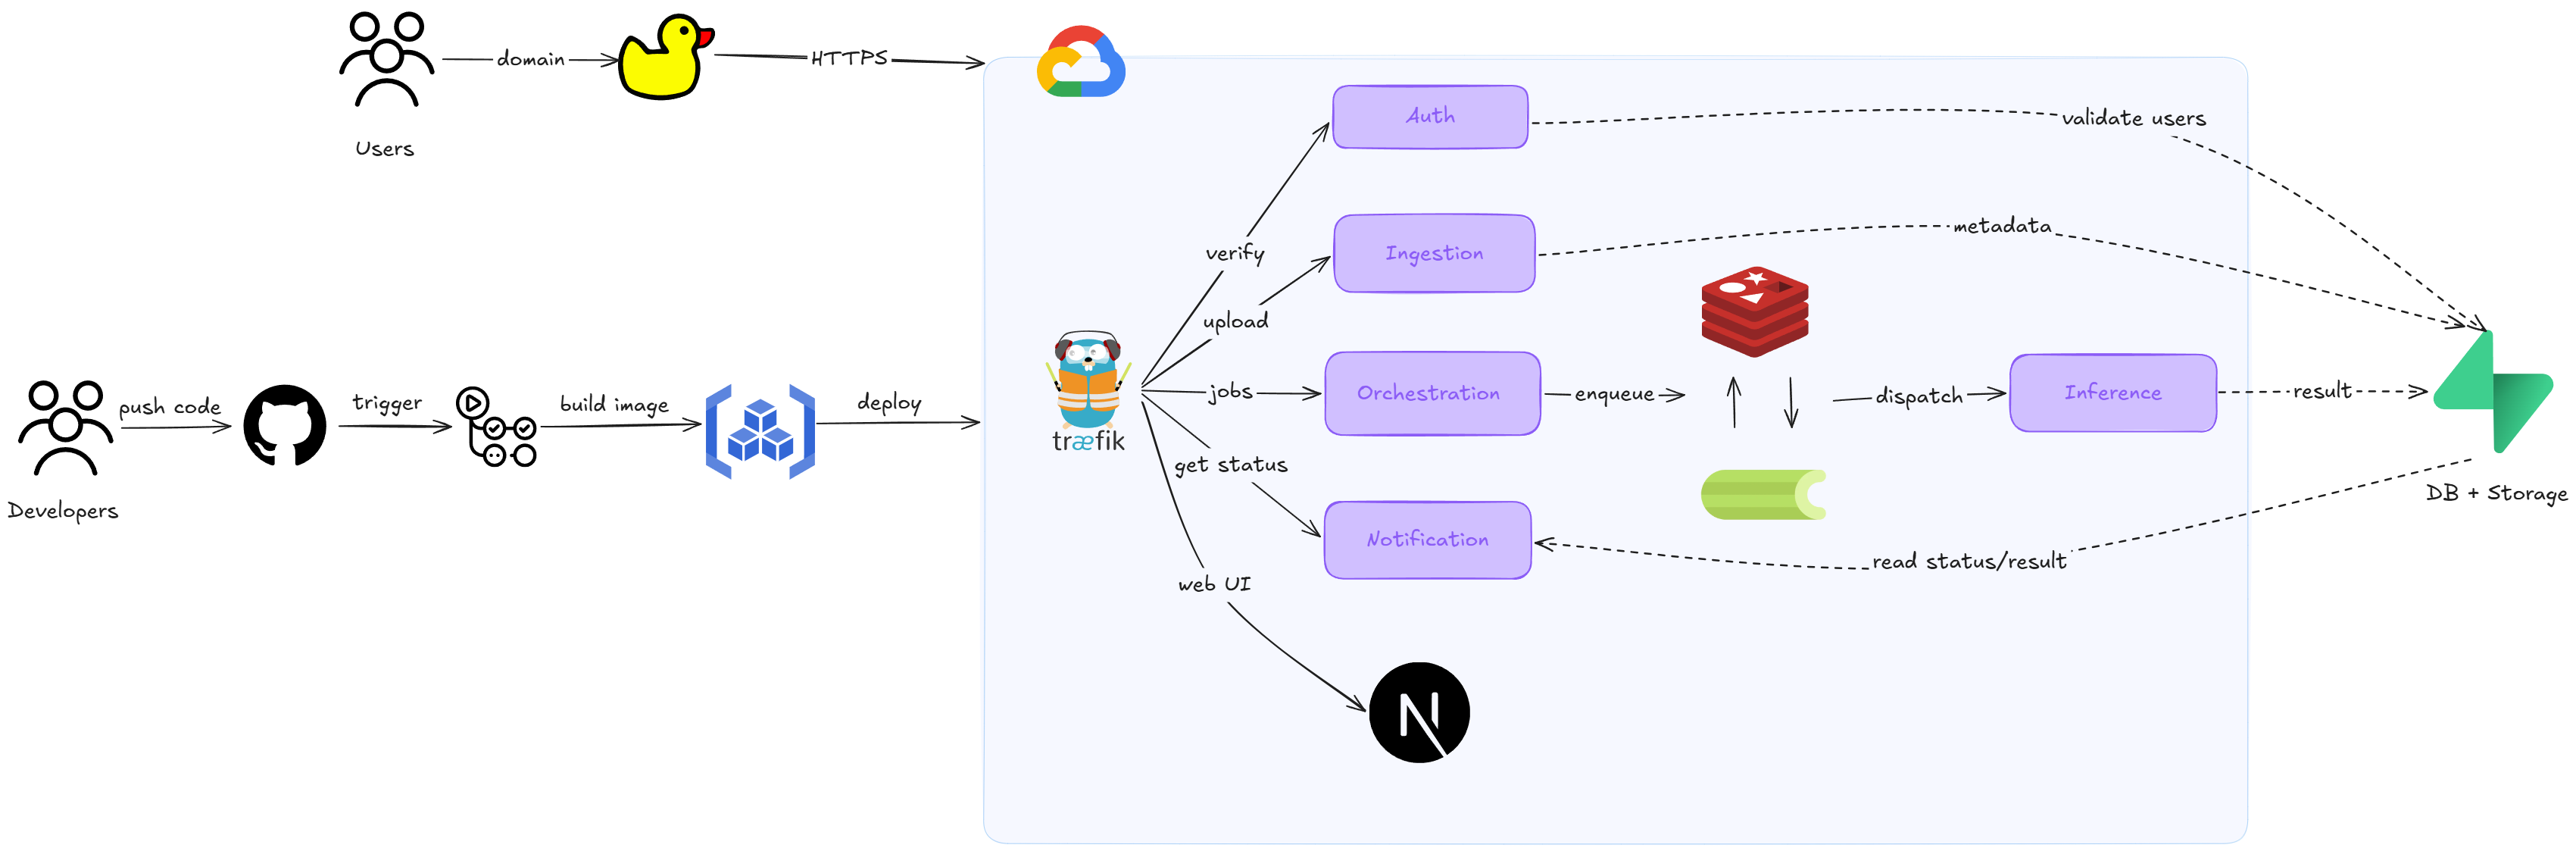
\includegraphics[width=\textwidth]{img/system_architecture.png}
    \caption{Kiến trúc triển khai của hệ thống phát hiện vi phạm không đội mũ bảo hiểm.}
    \label{fig:deployment-architecture}
\end{figure}

Người dùng truy cập hệ thống thông qua tên miền DuckDNS. Tên miền này trỏ đến điểm vào công khai của hệ thống trên Google Cloud, sau đó các yêu cầu HTTPS được định tuyến bởi Traefik. Traefik đóng vai trò như cổng vào chung, tiếp nhận các yêu cầu từ bên ngoài và chuyển tiếp đến đúng thành phần bên trong cụm triển khai.

Phần giao diện được xây dựng bằng Next.js và được triển khai như một container riêng. Các yêu cầu hiển thị trang web được Traefik định tuyến đến frontend. Các yêu cầu nghiệp vụ như đăng nhập, tải ảnh hoặc video, tạo tác vụ phát hiện và theo dõi trạng thái xử lý được chuyển đến các dịch vụ backend tương ứng.

Backend được tách thành nhiều dịch vụ theo chức năng. Dịch vụ Auth phụ trách xác thực người dùng và làm việc với Supabase Auth. Dịch vụ Ingestion tiếp nhận dữ liệu đầu vào, lưu tệp tải lên và metadata vào Supabase. Dịch vụ Orchestration tạo và quản lý các tác vụ phát hiện, sau đó đưa công việc vào Redis. Redis được sử dụng làm hàng đợi và bộ nhớ đệm trung gian. Inference Worker nhận tác vụ từ hàng đợi, chạy mô hình phát hiện vi phạm, sau đó ghi kết quả và đầu ra đã xử lý về Supabase. Dịch vụ Notification đọc trạng thái hoặc kết quả xử lý từ Supabase và cập nhật lại cho giao diện người dùng.

Supabase được đặt bên ngoài cụm Google Cloud và được sử dụng cho nhiều vai trò: cơ sở dữ liệu, xác thực, lưu trữ tệp và cập nhật thời gian thực. Cách tổ chức này giúp phần tính toán và phần triển khai ứng dụng nằm trên Google Cloud, trong khi dữ liệu người dùng, tệp đầu vào và kết quả được quản lý tập trung bởi Supabase.

\subsection{Giao diện và Chức năng}

Tại thời điểm viết báo cáo, nhóm chưa bổ sung ảnh chụp màn hình giao diện và chức năng thực tế của ứng dụng. Phần minh họa giao diện sẽ được cập nhật sau khi có ảnh chụp từ hệ thống đã triển khai.

\subsection{Triển khai}

Hệ thống được triển khai trên Google Cloud theo mô hình container hóa. Mỗi thành phần chính của ứng dụng, bao gồm frontend Next.js và các dịch vụ backend, được đóng gói thành Docker image. Khi lập trình viên đẩy mã nguồn lên GitHub, GitHub Actions được kích hoạt để xây dựng image, gắn nhãn theo commit SHA và đưa image lên Artifact Registry. Sau đó các workload trên Google Kubernetes Engine Autopilot được cập nhật để sử dụng phiên bản image mới.

Môi trường chạy trên Google Cloud sử dụng GKE Autopilot tại khu vực \texttt{asia-southeast1}. Traefik là điểm vào công khai duy nhất của hệ thống. Chứng chỉ TLS được cấp thông qua Let's Encrypt và cert-manager, giúp người dùng truy cập ứng dụng bằng giao thức HTTPS. Các dịch vụ nội bộ như Orchestration, Notification và Inference Worker không được mở trực tiếp ra Internet mà chỉ được gọi thông qua luồng định tuyến và giao tiếp nội bộ trong hệ thống.

Ứng dụng đã được gắn tên miền DuckDNS và có thể truy cập tại \href{https://dtdat-nthv.duckdns.org}{Helmet Violation Detection}.

Trong kiến trúc hiện tại, Supabase được sử dụng như dịch vụ bên ngoài cho cơ sở dữ liệu, xác thực, lưu trữ tệp và realtime. Redis được triển khai trong cụm Kubernetes để phục vụ hàng đợi tác vụ và bộ nhớ đệm. Cách triển khai này phù hợp với mục tiêu demo và staging ban đầu: giảm số lượng dịch vụ cloud phải quản lý, chỉ sử dụng một điểm vào công khai, và vẫn đảm bảo các thành phần chính của hệ thống có thể được triển khai, cập nhật và rollback thông qua pipeline CI/CD.
